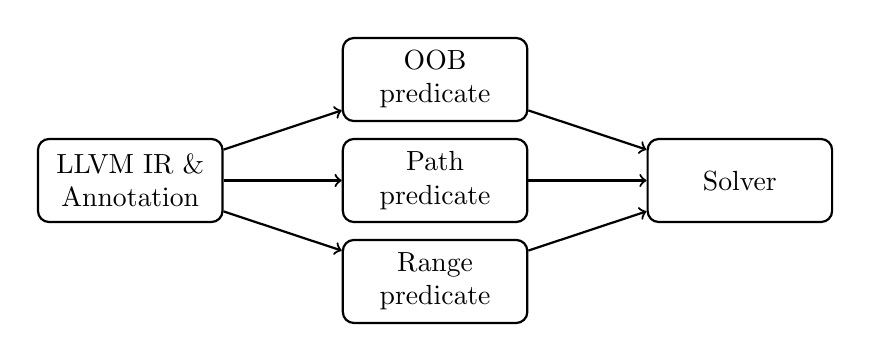
\begin{tikzpicture}[
	block/.style={
		rectangle, rounded corners,
		draw=black, thick,
		text width=6em, minimum height=3em, text centered
	},
	line/.style={draw, thick, ->},
	]
	\matrix[row sep=2mm, column sep=15mm] {
		& \node [block] (ec) {OOB predicate}; & \\
		\node [block, text width=6em] (ir) {LLVM IR \& Annotation};
		& \node [block] (pc) {Path\\predicate};
		& \node [block] (sol) {Solver}; \\
		& \node [block] (rc) {Range\\predicate}; & \\
	};

	\path [line] (ir) -- (ec);
	\path [line] (ir) -- (pc);
	\path [line] (ir) -- (rc);
	\path [line] (ec) -- (sol);
	\path [line] (pc) -- (sol);
	\path [line] (rc) -- (sol);
\end{tikzpicture}
